% Modelo de Dissertação em Latex para o PPG em Engenharia Mecânica da UERJ
% Este modelo foi adaptado da versão disponibilizada no site da Engenharia Elétrica da UERJ
% http://www.pel.uerj.br/publico/Modelo_LaTeX_Dissertacao_UERJ.rar
% http://www.pel.uerj.br/defesas/
%
% Utilizei o WinEdt 6.0 com Miktex 2.9
%
% Para gerar o PDF usei a opção PDFTeXfy com o documento [masterthesis.tex] aberto e em foco.
%
% Não consegui usar as figuras em EPS como o modelo original. Usei PNG e JPG sem problemas.
%
% Felipe M. - 20/06/2012
%
% 												Command             10pt    11pt    12pt
% 												\tiny               5       6       6
% 												\scriptsize         7       8       8
% 												\footnotesize       8       9       10
% 												\small              9       10      10.95
% 												\normalsize         10      10.95   12
% 												\large              12      12      14.4
% 												\Large              14.4    14.4    17.28
% 												\LARGE              17.28   17.28   20.74
% 												\huge               20.74   20.74   24.88
% 												\Huge               24.88   24.88   24.88


\documentclass[a4paper,12pt,oneside,openany]{uerj}
\usepackage[english,brazil]{babel}
% \usepackage[math]{iwona}
% \DeclareFontFamily{U}{futm}{}
% \DeclareFontShape{U}{futm}{m}{n}{
%   <-> fourier-bb % changed from .92 to 1
%   }{}
% \DeclareMathAlphabet{\mathbb}{U}{futm}{m}{n}
%\usepackage[latin1]{inputenc}
%\usepackage{fourier}
%\usepackage[utopia]{mathdesign}
%\usepackage{fouriernc}
%\usepackage{fontspec}
\usepackage{mathptmx} % Times New Roman

%\usepackage{Times}
\usepackage[T1]{fontenc}
\usepackage{lmodern}
%\setmainfont{Times}
%\setmainfont{Arial}
\usepackage[utf8]{inputenc}
\usepackage{enumerate}
\usepackage{cite}
\usepackage{epsf,epsfig,psfig}
\usepackage{pagina}
\usepackage{indentfirst}
\usepackage{theorem}
\usepackage{fancyhdr}
\usepackage{setspace}
\usepackage{boxedminipage}
\usepackage{float}
%\usepackage[style=base]{caption}
\usepackage{subcaption}
%\captionsetup{compatibility=false}
%\usepackage{subcaption}
%\usepackage[caption=false]{subfig}
\usepackage{silence}
\WarningFilter{caption}{Unsupported document class}
\usepackage{makeidx}
\usepackage{amsmath}
\usepackage{mathtools}
\usepackage{geometry}
\usepackage[hidelinks]{hyperref}
\pdfstringdefDisableCommands{\let\uppercase\relax} % desabilitar alguns warnings e \uppercase

%------------------------------------------------
\usepackage{xargs}                      % Use more than one optional parameter in a new commands
\usepackage[pdftex,dvipsnames]{xcolor}  % Coloured text etc.
\usepackage[colorinlistoftodos,prependcaption,textsize=normalsize]{todonotes}
\newcommandx{\balao}[2][1=]{\todo[linecolor=red,backgroundcolor=red!25,bordercolor=red,#1]{#2}}
\newcommandx{\change}[2][1=]{\todo[linecolor=blue,backgroundcolor=blue!25,bordercolor=blue,#1]{#2}}
\newcommandx{\info}[2][1=]{\todo[linecolor=OliveGreen,backgroundcolor=OliveGreen!25,bordercolor=OliveGreen,#1]{#2}}
\newcommandx{\improvement}[2][1=]{\todo[linecolor=Plum,backgroundcolor=Plum!25,bordercolor=Plum,#1]{#2}}
\newcommandx{\thiswillnotshow}[2][1=]{\todo[disable,#1]{#2}}
%------------------------------------------------
%------------------------------------------------
\usepackage{geometry}
\usepackage{mathtools}
\usepackage[version=4]{mhchem}
\usepackage{chemformula}
%------------------------------------------------

\makeindex


\newtheorem{deff}{Definição}[section]
\numberwithin{equation}{chapter}

\theoremstyle{plain}

\bibliographystyle{abnt-num}



\begin{document}

% \hypersetup{
%      colorlinks,
%     citecolor=black,
%     filecolor=black,
%     linkcolor=black,
%     urlcolor=black,
%     linktoc=all
% }

\thispagestyle{empty}\begin{titlepage}
\begin{center}

	\vspace{-0.5cm}

  \begin{figure}[hbt!]
		\begin{flushleft}
		   
\includegraphics[scale=0.3]{./00_Pre_textuais/logo_uerj_pb.png}
		\end{flushleft}
	\end{figure}
	\vspace{-4cm}

  \hspace{2cm}\large{\textbf{Universidade do Estado do Rio de Janeiro}}\\
  \hspace{2cm}\large{Centro de Tecnologia e Ciências}\\
  \hspace{2cm}\large{Faculdade de Engenharia}\\

  \hspace{2cm}\large{}\\
  \hspace{2cm}\large{}\\
  \hspace{2cm}\large{}\\
  \hspace{2cm}\large{}\\

  \par
  {\large{\authorName}}

  \hspace{2cm}\large{}\\
  \hspace{2cm}\large{}\\
  \hspace{2cm}\large{}\\
  \hspace{2cm}\large{}\\


  \par
  {\large\textbf{\mainTitle}}%Título do Trabalho


  \par\vfill
  Rio de Janeiro\\ \curYear

\end{center}
\end{titlepage}
\pagebreak\thispagestyle{empty}\begin{center}

\authorName

% \vfill
\vspace{2cm}

\textbf{\mainTitle}

\vspace{1.0cm}

\begin{figure}[hbt!]
\begin{center}

\includegraphics[width=10.48cm,height=10.8cm]{./00_Pre_textuais/logo_uerj_gnd_pb.png}
\end{center}
\end{figure}

\vspace{-9cm}
\begin{flushright}
\parbox{8cm}{
\singlespacing{Projeto Final apresentado a Faculdade de Engenharia da Universidade do Estado do Rio de Janeiro, para obtenção do grau de bacharel em Engenharia Mecânica}.
}
% \singlespacing{Dissertação apresentada, como requisito\linebreak parcial para obtenção do título de Mestre em Ciências, ao Programa de Pós-Graduação em Engenharia Mecânica, da Universidade do Estado do Rio de Janeiro. Área de\linebreak concentração: Fenômenos de Transporte}.
% }
\end{flushright}

\vspace{4.0cm}

Orientador: Prof. D.Sc. Gustavo R. Anjos\\

\par\vfill
%\vspace{2cm}

Rio de Janeiro\\ \curYear

\end{center}
\pagebreak\thispagestyle{empty}% Depois de preparar seu trabalho, você deverá enviá-lo para a Biblioteca CTC/B para avaliação do formato e elaboração da Ficha catalográfica.
% Com a ficha pronta (fornecida pela Biblioteca), você poderá alterar este trecho do trabalho em definitivo.
%
% Para este processo, enviei a dissertação em PDF para o email: ctcb.uerj.bdtd@gmail.com (Tratei de todos os detlahes com a Sra. Márcia)
% Qualquer dúvida, veja os contatos da Biblioteca no site da Rede Sirius: http://www.rsirius.uerj.br/
% 


\begin{titlepage}
	\begin{center}
\vfill
\singlespacing
	\vspace*{75mm}
	{CATALOGAÇÃO NA FONTE\\ \vspace{1.5mm}
	UERJ\,/\,REDE SIRIUS\,/\,BIBLIOTECA CTC/B}\\
	\vspace{1.5mm}
	\begin{boxedminipage}{140mm}
	\begin{minipage}{5mm}
		\vspace{-84mm}
		S237
	\end{minipage}
	\hfill
	\raisebox{8.5mm}{
	\begin{minipage}[top]{115mm}
		\vspace*{5mm}

		Sobrenome, Nome do Autor\\
		\phantom{XX}Título\,/\,Nome completo do autor. -- 2018.\\
		\phantom{XX}105\,f.\\
		\phantom{XX}\\
		\phantom{XX}Orientadores: Nome completo do orientador1;\\
\hspace*{5mm}
Nome completo do orientador2\\
       		\phantom{XX}Projeto Final (Bacharel em Engenharia Mecânica) -- Universidade do Estado do Rio de Janeiro, Faculdade de Engenharia.\\
		\phantom{XX}\\
		\phantom{XX}Texto a ser informado pela biblioteca.
	\end{minipage}}
	\vspace*{5mm}
	\begin{flushright}
	 CDU~621:528.8
	\end{flushright}
    \vspace{1mm}
	\end{boxedminipage}\\
	\end{center}
%
	Autorizo, apenas para fins acadêmicos e científicos, a reprodução total ou parcial deste projeto final, desde que citada a fonte.\\
	\noindent
	\begin{tabular}{ccc}
	\phantom{XXXXXXXXXXXXXXXXXXXXXXXXXXXXXX}&	 \phantom{XX}	&	\phantom{XXXXXXXXXXXXXXXX}	\\
	\phantom{XXXXXXXXXXXXXXXXXXXXXXXXXXXXXX}&	 \phantom{XX}	&	\phantom{XXXXXXXXXXXXXXXX}	\\
	\cline{1-1}\cline{3-3}
	Assinatura &		&	Data
	\end{tabular}
\end{titlepage}   
\pagebreak\thispagestyle{empty}\addtocounter{page}{+1}
\begin{center}

\authorName

\vspace{1cm}

\textbf{\mainTitle}

\end{center}

\vspace{.4cm}

\begin{flushright}
\small{\parbox{8cm}{
\singlespacing{Projeto Final apresentado a Faculdade de Engenharia da Universidade do Estado do Rio de Janeiro, para obtenção do grau de \linebreak bacharel em Engenharia Mecânica}.
% \singlespacing{Dissertação apresentada, como requisito\linebreak parcial para obtenção do título de Mestre em Ciências, ao Programa de Pós-Graduação em Engenharia Mecânica, da Universidade do Estado do Rio de Janeiro. Área de\linebreak concentração: Fenômenos de Transporte}.
}}
\end{flushright}

\vspace{.6cm}


% insira abaixo a data de sua defesa
% Caso não tenha defendido ainda, deixe em branco

\noindent Aprovado em: 25 de Junho de 2019 %29 de Maio de 2018

\noindent Banca Examinadora:


%
%
% Os professores da UERJ DEVEM ser citados primeiro, independente de quem seja o orientador.
%
%



\vspace{.7cm}

\begin{flushright}
\parbox{12cm}{

\singlespacing

\hrulefill \\

\vspace{-.4cm}
Prof. D.Sc. Gustavo R. Anjos - Orientador
\newline
Universidade Federal do Rio de Janeiro - UFRJ - COPPE
\vspace{.7cm}

\hrulefill \\

\vspace{-.4cm}
Prof. D.Sc. Norberto Mangiavacchi
\newline
Departamento de Engenharia Mecânica - UERJ
\vspace{.7cm}

\hrulefill \\

\vspace{-.4cm}
Prof. D.Sc. Fábio Pereira dos Santos
\newline
Universidade Federal do Rio de Janeiro - UFRJ - COPPE
\vspace{.7cm}

\hrulefill \\

\vspace{-.4cm}
D.Sc. Leon Matos Ribeiro de Lima
\newline
Eletronuclear
\vspace{.7cm}

% \hrulefill \\

% \vspace{-.4cm}
% Prof. Dr. Nome do Professor 5
% \newline
% Universidade Federal do Rio de Janeiro - UFRJ - COPPE
% \vspace{.7cm}

}
\end{flushright}
\vfill

\begin{center}
Rio de Janeiro\linebreak \curYear
\end{center}
\pagebreak\thispagestyle{empty}\begin{center}
\textbf{DEDICATÓRIA}
\end{center}

$\!$\\

%\vspace{1cm}

Aqui entra sua dedicatória.
\pagebreak\thispagestyle{empty}\begin{center}
\textbf{AGRADECIMENTO}
\end{center}

Agradeço aos meus pais, Luis Sousa e Elizabeth Carvalho, que sempre me apoiaram, serviram de inspiração e como excelentes exemplos que sempre segui com orgulho.

A minha companheira, Juliana Marques, pelo carinho e apoio sempre que precisei.

A meus orientadores, Gustavo Rabello dos Anjos, pelo apoio e incentivo, e Leandro Marques, pela ajuda na organização, planejamento e revisão do texto.

A meu avô Mario Carvalho, pela inspiração e por me mostrar a engenharia de perto. E a minha tia Tathiana Carvalho, pela ajuda com o texto.

Finalmente, aos meus amigos Daniel Coelho, Luís Carnevale, Douglas Lopes, Thiago Cabral e todos os outros que me ajudaram no período da graduação, dentro e fora da sala de aula.
%\pagebreak\thispagestyle{empty}$\!$\\
$\!$\\
$\!$\\
$\!$\\
$\!$\\
$\!$\\
$\!$\\
$\!$\\
$\!$\\
$\!$\\
$\!$\\
$\!$\\
$\!$\\
$\!$\\
$\!$\\
$\!$\\
$\!$\\
$\!$\\
$\!$\\
$\!$\\
$\!$\\
$\!$\\

\begin{flushright}
\textit{xxxxxxxxxxxxx xxxxxxxx xxxxxxxxx}
\end{flushright}
\vspace{-1cm}
\begin{flushright}
\textit{xxxxxxxxxxxxx xxxxxxxxx}
\end{flushright}
\begin{flushright}
John Doe
\end{flushright}

\thispagestyle{empty}    % não coloquei epígrafe no meu trabalho, mas fica aqui a chamada comentada.
\pagebreak\thispagestyle{empty}\begin{center}
\textbf{RESUMO}
\end{center}

%
% O resumo deve ser organizado em apenas um parágrafo mesmo.
% O número de folha é o número de páginas do PDF -2. Isto ocorre pois na versão final (capa dura) a capa é removida e as duas primeiras páginas são impressas em uma % folha apenas (frente e verso).
%

$\!$\\

\hspace{-1.3cm}\textbf{SOUSA}, Lucas Carvalho de. \textit{\mainTitle}. \numPages. Projeto Final~(Bacharelado em Engenharia Mecânica) - Faculdade de Engenharia, Universidade do Estado do Rio de Janeiro~(UERJ), Rio de Janeiro, \curYear.

\vspace{.2cm}

Aqui entra o seu resumo organizado em um parágrafo apenas.

\vspace{1cm}

\hspace{-1.3cm}Palavras-chave: Método de Elementos Finitos, Formulação Corrente-Vorticidade, Escoamento Multifásico, Escoamento Particulado.
\pagebreak\thispagestyle{empty}\begin{center}
\textbf{ABSTRACT}
\end{center}

$\!$\\

% O resumo em inglês deve ser organizado em apenas um parágrafo mesmo.

Aqui entra seu resumo em inglês também organizado em apenas um parágrafo.

\vspace{1cm}

\hspace{-1.3cm}Keywords: Pattern Formation, Swift-Hohenberg Equation, Computacional Modelling, Word4.

\fancypagestyle{plain}{
\fancyhf{} % clear all header and footer fields
\renewcommand{\headrulewidth}{0pt}
\renewcommand{\footrulewidth}{0pt}}
\pagestyle{plain}

\pagebreak

\def\listfigurename{LISTA DE FIGURAS}\listoffigures
\def\listtablename{LISTA DE TABELAS}\listoftables
\newpage

\begin{center}
\textbf{LISTA DE ABREVIATURAS E SIGLAS}
\end{center}
$\!$\\

\begin{tabular}{lll}
MEF & \hspace{1cm} & Método de Elementos Finitos \\
MDF & \hspace{1cm} & Método das Diferenças Finitas \\
POO &  \hspace{1cm} & Programação Orientada a Objeto \\
BBO &  \hspace{1cm} & Equação de Basset–Boussinesq–Oseen \\
% ANN & \hspace{1cm} & Artificial Neural Network \\
% AOA&  \hspace{1cm} &Angle of Arrival \\
% AP&  \hspace{1cm} &Access Point \\
% BCCH&  \hspace{1cm} &Broadcast Control Channel \\
\end{tabular}    % não coloquei LISTA DE SIGLAS no meu trabalho, mas fica aqui a chamada comentada.
\def\contentsname{SUMÁRIO}\tableofcontents

\fancypagestyle{plain}{
\fancyhf{} % clear all header and footer fields
\fancyhead[R]{\thepage}
\setlength{\voffset}{-1cm}
\setlength{\headsep}{1cm}
\renewcommand{\headrulewidth}{0pt}
\renewcommand{\footrulewidth}{0pt}}

\pagestyle{plain}

\pagebreak
\addcontentsline{toc}{chapter}{\hspace{1.7cm}\bfseries INTRODUÇÃO}
\noindent\textbf{INTRODUÇÃO}
$\!$\\
\indent Os problemas físicos de interesse da engenharia mecânica, muitas vezes, podem se apresentar de forma multidisciplinar e em razão disso também oferecem resultados que exigem ferramental e perspectivas oferecidos por outras disciplinas e áreas não contempladas em um curso usual de um engenheiro mecânico. Um desses problemas é o fenômeno de difusão acompanhado de reações químicas (homogêneas ou heterogêneas), em geral não lineares, que, em condições conhecidas, configuram processos de organização espacial de substâncias ou espécies. Por exemplo, reações químicas autocatalíticas ou outros tipos de interações em sistemas difusivos com mais de uma substâncias ou espécies, e.g., o caso particular de auto-organização dentro de uma classe mais ampla conhecida como estruturas dissipativas: padrões (estruturas) de turing.\par
\begin{figure}[H]
\centering
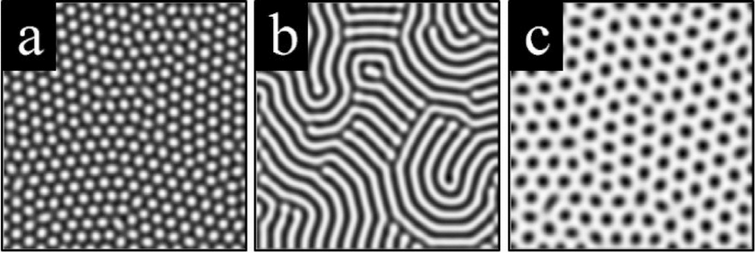
\includegraphics[scale=0.5]{01_Pre_textuais/turing2.PNG}
\end{figure}
As equações de reação-difusão são conhecidas por modelarem fenômenos químicos e biológicos, os quais, se originam da interação entre indivíduos, células ou espécies. A modelagem matemática desses mecanismos tem sido bem sucedida e vem se desenvolvendo em áreas como ecologia, embriologia (morfogênese), neurobiologia, \textcolor{red}{outros}, bem como cinéticas químicas no estado sólido. Este último tema é de interesse da ciência dos materiais computacional, uma vez que modelos matemáticos de problemas físicos tais como crescimento dendrítico (evolução cristalina), formação de precipitados em ligas metálicas e cerâmicas ou até mesmo transformação de fase por avanço de frente tornam-se possíveis.\par
Padrões espaço-temporais se apresentam em diversos âmbitos da natureza e sua descrição e compreensão ainda levantam questões importantes e básicas. Comparando com cerca de 30 anos atrás, grande progresso foi conquistado na modelagem de instabilidades, análise da dinâmica na vizinhança, formação e estabilidade de padrões, análise quantitativa experimental e numérica de padrões, e assim por diante. \par
Modelos de Reação-Difusão podem evoluir para um padrão
espacial heterogêneo e estável ao longo do tempo devido a pequenas perturbações das
concentrações das substâncias químicas em relação a um estado de equilíbrio espacial
homogêneo.\par
% Comportamentos universais de sistemas complexos próximos a instabilidades foram determinados, levando à ampla interdisciplinaridade de um campo que agora é chamado de ciência não-linear ou ciência da complexidade, e no qual conceitos iniciais de estruturas dissipativas ou sinergéticas estão profundamente enraizados.\par
% Em domínios pioneiros relacionados à hidrodinâmica ou às instabilidades químicas, as interações entre experimentalistas e teóricos, às vezes cotidianamente, têm sido fundamentais para o progresso. Todos no campo elogiam o papel desempenhado pelas interações e retornos permanentes entre estudos experimentais, numéricos e analíticos nas conquistas obtidas durante esses anos. Muitos aspectos de padrões convectivos em fluidos normais, misturas binárias ou cristais líquidos são agora entendidos e descritos neste contexto. A presença genérica de defeitos em sistemas estendidos está agora bem estabelecida e induziu novos desenvolvimentos na física de laser com grandes números de Fresnel. Por último, mas não menos importante, quase 40 anos depois de seu célebre trabalho, as estruturas de Turing foram finalmente obtidas em reatores químicos da vida real, desencadeando uma nova atividade intensa no campo dos sistemas de reação-difusão.
\textcolor{red}{Posicionar histórico, experiências, resultados, modelos, referências, etc. As teorias matemáticas...}
% \begin{figure}[H]
% \centering
% 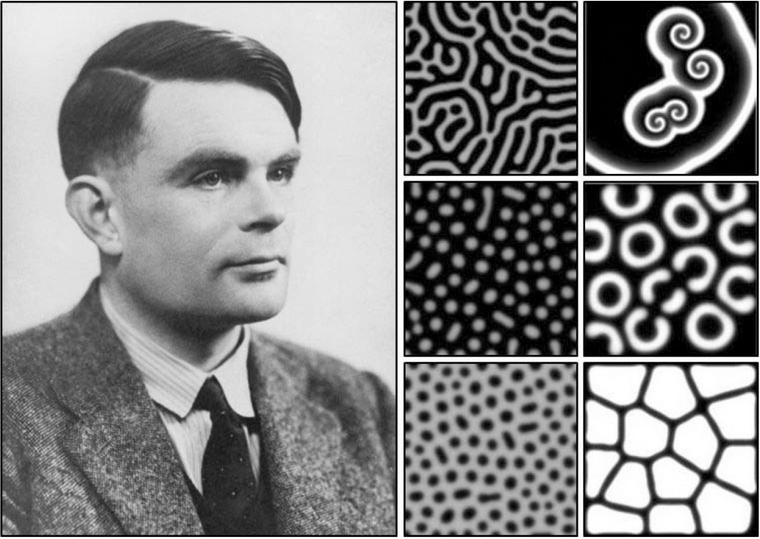
\includegraphics[scale=0.4]{01_Pre_textuais/turing1.PNG}
% \end{figure}
% \textcolor{red}{Posicionar referências}

\chapter{REVISÃO DA LITERATURA}
\label{cap1}
\section{\textbf{Introdução}}

Tópicos:
\textcolor{red}{  
\begin{itemize}
    \item O papel do estudo da formação de padrões na eng mec
    \item Background teórico e disciplinas/áreas necessárias
    \item Casos de interesse
\end{itemize}}

\section{\textbf{Reações-difusão em ciência dos materiais}}


% \section{\textbf{Motivação do Projeto}}

% O reconhecimento de que o fenômeno difusional está presente em muitos âmbitos de diversos problemas físicos nos leva ao questionamento de como ou porque outros fenômenos ocorrem envolvendo ou em função deste.

% \section{\textbf{Organização do Projeto}}
% Além do presente capítulo, o projeto encontra-se organizado em outros seis como descritos abaixo.\\
% \noindent\textbf{Capítulo 2}\par
% Neste capítulo \\
% \noindent\textbf{Capítulo 3}\par
% Neste capítulo são apresentados...\\
% \noindent\textbf{Capítulo 4}\par
% Neste capítulo são apresentados...\\
% \noindent\textbf{Capítulo 5}\par
% Neste capítulo são apresentados...\\
% \section{\textbf{Conclusão}}



\chapter{Sistemas Não Lineares}
\label{chapter:cap3}
\section{\textbf{Introdução}}

\section{\textbf{Modelo de \textit{Lorenz}}}
\begin{figure}[H]
%     \centering
    \begin{subfigure}{.5\textwidth}
    \centering
    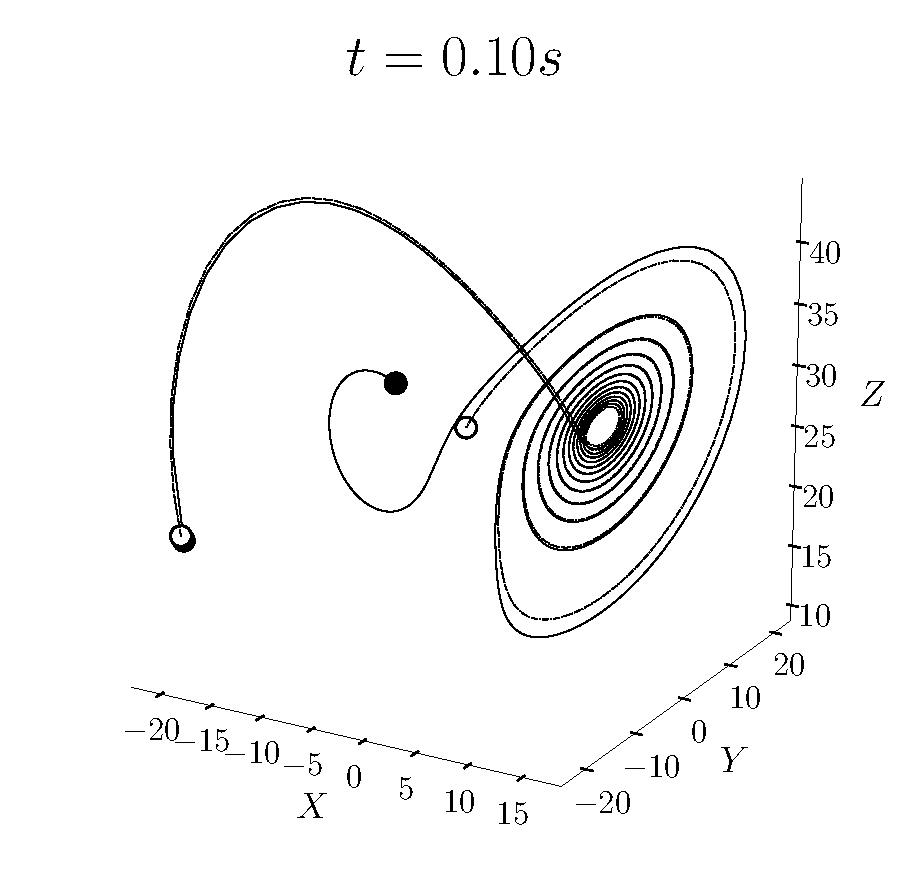
\includegraphics[width=1.\linewidth, angle=0, clip]{03_Cap3/figures/Lorenzatractor0_10.pdf}
    \end{subfigure}
    \begin{subfigure}{.5\textwidth}
    \centering
    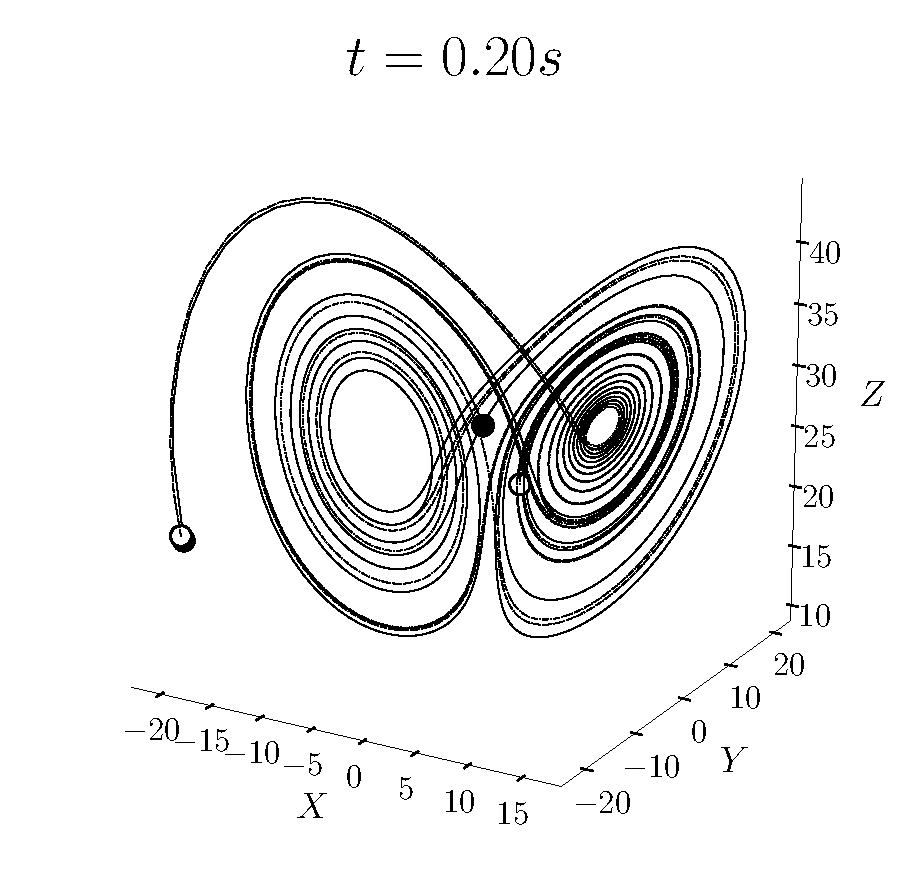
\includegraphics[width=1.\linewidth, angle=0, clip]{03_Cap3/figures/Lorenzatractor0_20.pdf}
    \end{subfigure}
    \vspace{-0.5cm}
\end{figure}
\section{\textbf{Mecanismo de reações: \textit{Brusselator}}}
O Mecanismo proposto por Prigogine e Levefer em 1968 consiste na sequência de reações em \ref{brureactions}, da qual, através da \textit{Lei de Ação das Massas}, obtemos o sistema de equações diferenciais ordinárias \ref{brusys}:\\
\begin{minipage}{.48\textwidth}
\vspace{-3ex}
\begin{align}
\hspace{-10pt}
\centering
\overline{A}&\ce{->T[\ce{$k_1$}]}\overline{X} \nonumber\\
\overline{B}+\overline{X}&\ce{->T[\ce{$k_2$}]}\overline{Y}+\overline{D} \nonumber\\
2\overline{X}+\overline{Y}&\ce{->T[\ce{$k_3$}]}3\overline{X} \nonumber\\
\overline{X}&\ce{->T[\ce{$k_4$}]}\overline{E} 
\label{brureactions}
\end{align}
\end{minipage}
\begin{minipage}{.04\textwidth}
\vspace{-3ex}
\end{minipage}
\begin{minipage}{.48\textwidth}
\vspace{-3ex}
\begin{equation}
\centering
%\text{simult\'aneas:}\quad
    \begin{dcases}
      \frac{d\overline{X}}{dt}=k_{1}\overline{A}-(k_{2}\overline{B}+k_{4})\cdot\overline{X}+k_{3}\overline{X}^2\cdot\overline{Y}\\
      \frac{d\overline{Y}}{dt}=k_{2}\overline{B}\cdot\overline{X}-k_{3}\overline{X}^2\cdot\overline{Y}\\
    \end{dcases}
%     \quad
%     \Leftrightarrow
%     \quad
%     x=1,~y=1
\label{brusys}
\end{equation}
\end{minipage}
\\[2ex]
% $\!$\\
% \vspace{2ex}
Admensionalizando as equações da forma a seguir, obtemos:
\begin{equation*}
\centering
    \begin{dcases}
      \frac{dX}{dt}=A-(B+1)X+X^2Y\\
      \frac{dY}{dt}=BX-X^2Y\\
    \end{dcases}
\end{equation*}

\subsection{Análise de estabilidade linear}
\textcolor{red!}{Escrever análise, condição de estabilidade, ponto fixo e regimes estáveis, instáveis, focos estáveis, instáveis.... }

\begin{figure}[H]
%     \centering
    \begin{subfigure}{.5\textwidth}
    \centering
    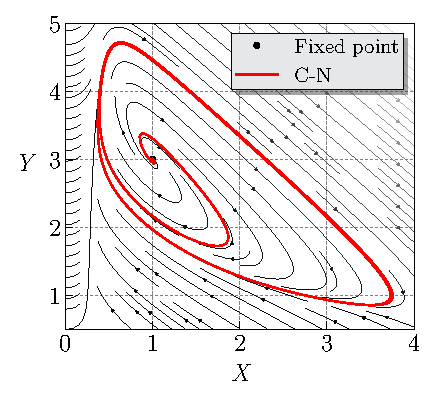
\includegraphics[width=1.\linewidth, angle=0, clip]{03_Cap3/figures/Phase_Space_internal__Brusselator__CN.pdf}
    \end{subfigure}
    \begin{subfigure}{.5\textwidth}
    \centering
    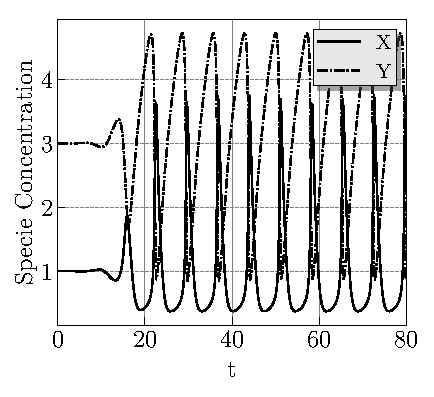
\includegraphics[width=1.\linewidth, angle=0, clip]{03_Cap3/figures/Temporal_evolution_internal__Brusselator__CN.pdf}
    \end{subfigure}
    \vspace{-0.5cm}
\end{figure}
\begin{figure}[H]
% 	\centering
	\vspace{-0.5cm}
    \begin{subfigure}{.5\textwidth}
    \centering
    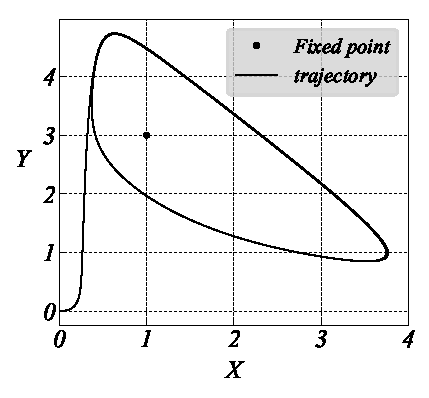
\includegraphics[width=1\linewidth, angle=0, clip]{03_Cap3/figures/Phase_Space_external__Brusselator__CN.pdf}
    \end{subfigure}
    \begin{subfigure}{.5\textwidth}
    \centering
    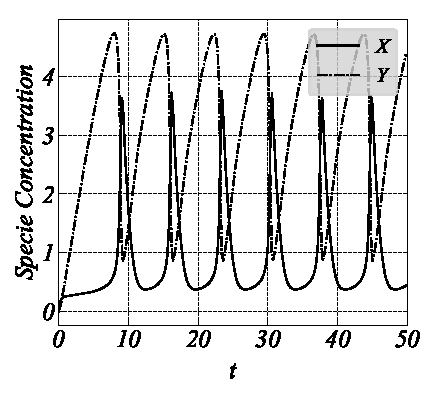
\includegraphics[width=1\linewidth, angle=0, clip]{03_Cap3/figures/Temporal_evolution_external__Brusselator__CN.pdf}
    \end{subfigure}
    \vspace{-0.5cm}
\end{figure}



\section{\textbf{Equação de \textit{Van der Pol}}}
\textcolor{red!}{(Ver Appendix 3 do Murray, Jordan and Smith 1987, Liénard Equation)}\par
A equação de \textit{Van der Pol} modela matematicamente um oscilador cujo termo de amortecimento é não linear. A equação diferencial ordinária de $2^{a}$ ordem (\ref{vanderpol}) pode ser subdividida em um sistema de EDO's de $1^{a}$ ordem (\ref{vanderpolsys}).
\begin{equation}
\ddot{x}+\epsilon (x^{2}-1)\dot{x}+x=0
\label{vanderpol}
\end{equation}
\begin{equation}
\centering
    \begin{dcases}
      \frac{dx}{dt}=y\\
      \frac{dy}{dt}=\epsilon (1-x^{2})y-x\\
    \end{dcases}
\label{vanderpolsys}
\end{equation}



\begin{figure}[H]
% 	\centering
	\vspace{-0.5cm}
    \begin{subfigure}{.5\textwidth}
    \centering
    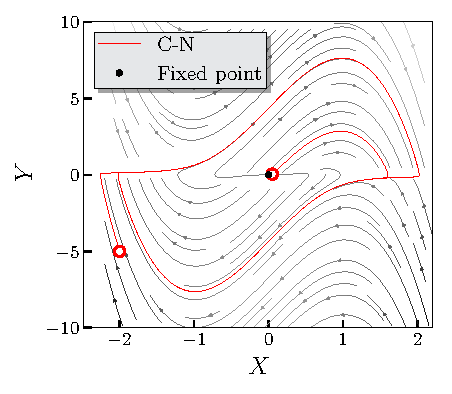
\includegraphics[width=1.\linewidth, angle=0, clip]{03_Cap3/figures/VanderPol2__Phase_Space_ep5.pdf}
    \end{subfigure}
    \begin{subfigure}{.5\textwidth}
    \centering
    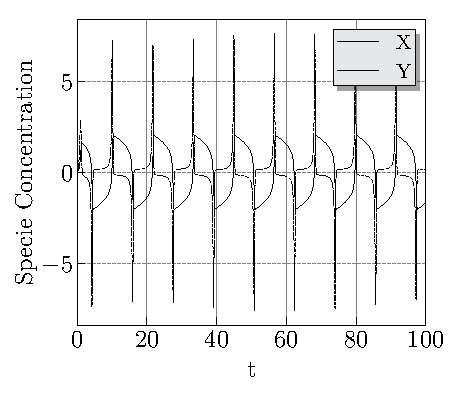
\includegraphics[width=1.\linewidth, angle=0, clip]{03_Cap3/figures/VanderPol2__2nd_Time_Evolution_ep5.pdf}
    \end{subfigure}
    \vspace{-0.5cm}
\end{figure}


% Equação...
% \begin{figure}[H]
%     \begin{subfigure}{.5\textwidth}
%     \centering
%     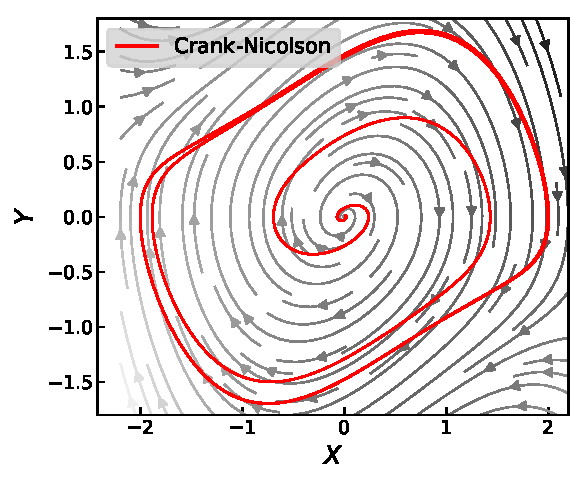
\includegraphics[width=1.0\linewidth, angle=0, clip]{02_Cap2/figures/VanderPol__Phase_Space_.pdf}
%     \end{subfigure}
%     \begin{subfigure}{.5\textwidth}
%     \centering
%     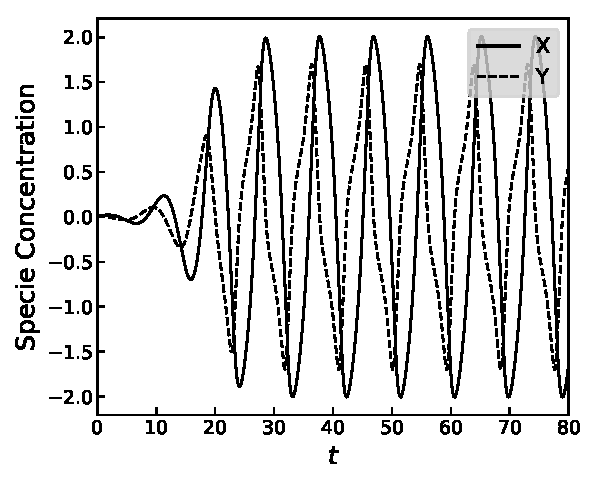
\includegraphics[width=1.0\linewidth, angle=0, clip]{02_Cap2/figures/VanderPol__Time_Evolution_.pdf}
%     \end{subfigure}
%     \vspace{-0.5cm}
% \end{figure}
% \begin{figure}[H]
%     \begin{subfigure}{.5\textwidth}
%     \centering
%     \includegraphics[width=1.0\linewidth, angle=0, clip]{02_Cap2/figures/VanderPol2__Phase_Space_.pdf}
%     \end{subfigure}
%     \begin{subfigure}{.5\textwidth}
%     \centering
%     \includegraphics[width=1.0\linewidth, angle=0, clip]{02_Cap2/figures/VanderPol2__Time_Evolution_.pdf}
%     \end{subfigure}
%     \vspace{-0.5cm}
% \end{figure} 

\section{\textbf{Modelo de \textit{Fitz-Hugh Nagumo}}}
Um dos modelos estudados extensivamente em neurobiologia e utilizado para teoria de membranas nervosas de Hodgkin-Huxley.







%\chapter{Outro Cap}
\label{chapter:cap4}

\section{\textbf{Introdução}}
Neste capítulo apresenta-se uma classificação dos métodos de localização bidimensional de MS em redes de telefonia móvel celular. Esta classificação simplificada utiliza apenas três critérios: o método de cálculo, o grau de participação do MS no cálculo de posição e o número mínimo de setores requerido para 

\section{\textbf{Conceitos Básicos}}
\label{sec:Cap1Conceitos}

Alguns conceitos que serão utilizados na descrição dos métodos de localização precisam ser previamente definidos.


\begin{figure}[H]
\begin{center}
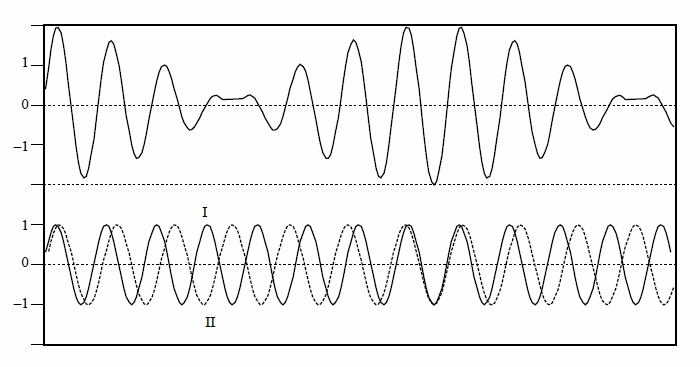
\includegraphics[width=8cm,height=6.4cm]{./01_Cap1/figures/fig_06_br.png}
\caption{\label{fig:bestserverarea}- Áreas Preditas de Melhor Servidor de Três Setores.}
\end{center}
\end{figure}

\section{\textbf{Classificação segundo o Método de Cálculo}}
\label{sec:Cap1Metodo}

O primeiro critério de classificação é a maneira pela qual os métodos de localização calculam a estimativa de posição do MS no plano. Para utilizar a geometria euclidiana, é necessário que as coordenadas geográficas dos setores de referência e do MS sejam representadas através uma projeção cartográfica retangular, ou 

\subsection{Identidade da Célula}
\label{subsec:Cap1Cid}

No método de localização da identidade da célula~(CID - \textit{Cell Identity}), a posição do MS é assumida como sendo igual à da antena transmissora do setor melhor servidor. O método CID, embora seja de baixa complexidade e elevada 

\subsection{Triangulação}
\label{subsec:Cap1Triangulacao}

As técnicas de triangulação utilizam medidas de distâncias~(multi-lateração) ou ângulos~(multi-angulação) entre o MS e os setores de referência para estimar a localização do 

Todos os métodos de triangulação presumem condições de propagação com linha de visada~(LOS - \textit{Line of Sight}) entre o MS e setores de referência. A propagação por múltiplos percursos e a presença de obstáculos entre o MS e os setores de referência podem corromper as medidas angulares, de tempo e de atenuação no percurso. Assim, a propagação sem linha de visada~(NLOS - \textit{Non Line of Sight}) é a principal fonte de erro para esses métodos. Como a propagação NLOS predomina em ambientes urbanos, a precisão dos métodos de triangulação pode ser seriamente comprometida nesses ambientes.

Além da propagação NLOS, outro fator que limita a precisão dos métodos de triangulação é a resolução finita das medidas realizadas na interface aérea e que são utilizadas no cálculo de posição: tempo, RSS e ângulo de chegada. A resolução da medida de RSS depende de especificações da interface rádio. Em redes GSM e WCDMA, por exemplo, os valores de RSS são reportados pelo MS em passos de $1$ dB~\cite{MURRAY}
\begin{equation}
\label{eq:dist}
\hat{d}_{i}= \frac{c \cdot \textrm{T}_{s} \cdot \textrm{RTT}_{i}}{2}
\end{equation}


\begin{table}[ht]
\centering
\caption{\label{tab:quadrosinotico}- Quadro Sinótico dos Métodos de Localização.}
\vspace*{.1cm}
\begin{scriptsize}
\begin{tabular}{|c|c|c|c|c|c|}
\hline
\textbf{Sigla} & \textbf{Método de Cálculo} & \textbf{Participação} & \textbf{Quant. Mín.} & \textbf{Elem. adicionais} & \textbf{Requer}\\
& & \textbf{do MS} & \textbf{de Setores} & \textbf{na RAN} & \textbf{LOS ?}\\
\hline
AOA	& Triang. por multi-angulação & Baseado & 2	& Conj. de antenas & Sim \\
& & na Rede & & diretivas & \\
\hline
CID	& Identidade da célula	& Baseado & 1	& - & Não\\
& & na Rede & & & \\
\hline
EOTD	& Triang. por multi-lateração &	Assistido ou &	3	& LMUs & Sim \\
& hiperbólica & Baseado no MS & & & \\
\hline
AGPS	& Triang. por multi-lateração & Assistido & 3 & - & Sim \\
& circular & pelo MS & & & \\
\hline
CID+RTT	& Triang. por multi-lateração &	Baseado & 3	& - & Sim \\
& circular com RTT & na Rede & & & \\
\hline
CID+RSS	& Triang. por multi-lateração circular  &	Baseado & 3	& - & Sim \\
& com perda de propagação & na Rede & & & \\
\hline
AOA+RTT	& Híbrido	& Baseado & 1	&  Conj. de antenas & Sim \\
& & na Rede & & diretivas & \\
\hline
AOA+RSS	& Híbrido	& Baseado & 1	&  Conj. de antenas & Sim \\
& & na Rede & & diretivas& \\
\hline
AOA+TDOA	& Híbrido	& Assistido & 2	&  Conj. de antenas & Sim \\
& & pelo MS & & diretivas& \\
\hline
\end{tabular}
\end{scriptsize}
\vspace*{-.2cm}
\end{table}




\chapter{Mecanismos de Reação-Difusão}
\label{chapter:cap5}
\section{\textbf{Introdução}}


\section{\textbf{Equação de Reação-Difusão: \textit{Fitz-Hugh Nagumo}}}

\section{\textbf{Equação de Reação-Difusão: \textit{Belousov-Zhabotinski}}}
Reação oscilatória importante descoberta por...
\begin{flalign*}
\hspace{-10pt}
\centering
\overline{A}+\overline{Y}&\ce{->T[\ce{$k_1$}]}\overline{X}+\overline{P}\;,\quad \overline{X}+\overline{Y}\ce{->T[\ce{$k_2$}]}2\overline{P}\\
\overline{A}+\overline{X}&\ce{->T[\ce{$k_3$}]}2\overline{X}+2\overline{Z}\;,\quad 2\overline{X}\ce{->T[\ce{$k_4$}]}\overline{A}+\overline{P}\;, \quad \overline{Z}\ce{->T[\ce{$k_5$}]}f\overline{Y}\\
\end{flalign*}

% \chapter{Implementação Numérica}
\label{chapter:cap6}
\section{\textbf{Introdução}}
\section{\textbf{Linguagem de Programação \textit{Python}}}
\section{\textbf{Método de \textit{Splitting}}}
\subsection{Discretização Espacial}
\subsection{Discretização Temporal (\textit{Crank-Nicolson})}

\chapter{Modelagem Matemática e Esquema numérico}
\label{chapter:cap2}
\section{\textbf{Equação governo}}
\section{\textbf{Parâmetros realísticos}}


%\chapter{Implementação Numérica}
\label{chapter:cap7}
\section{\textbf{Introdução}}
\section{\textbf{Linguagem de Programação Python}}

\chapter{Verificação e Estabilidade}
\label{chapter:cap8}
\section{\textbf{Verificação do código}}
\section{\textbf{Convergência e erro}}
\section{\textbf{Estabilidade do esquema}}

\chapter{Resultados}
\label{chapter:cap9}
\section{\textbf{Preliminares}}
\section{\textbf{Avançados}}

% \chapter{Implementação Numérica}
\label{chapter:cap7}
\section{\textbf{Introdução}}
\section{\textbf{Linguagem de Programação Python}}


% inserir demais capítulos aqui
% -----------------------------
% -----------------------------
% -----------------------------
% -----------------------------





\pagebreak
\addcontentsline{toc}{chapter}{\hspace{1.7cm}\bfseries CONCLUSÃO}
\noindent\textbf{CONCLUSÃO}
$\!$\\

Aqui entra sua conclusão!!

\pagebreak
\addcontentsline{toc}{chapter}{\hspace{1.7cm}\bfseries APÊNDICE A}
\setcounter{section}{0}
\setcounter{chapter}{0}%
 \renewcommand{\theequation}{A.\arabic{equation}}    
  % redefine the command that creates the equation no.
% \renewcommand{\thechapter}{\arabic{chapter}}%
\noindent\textbf{APÊNDICE A - SOLUÇÃO NUMÉRICA DA EQUAÇÃO DO CALOR BIDIMENSIONAL E VALIDAÇÃO DO CÓDIGO}
$\!$\\

% Nesse apêndice são desenvolvidas e executadas duas formas de solucionar 
% numericamente equações diferenciais parciais que possuem o termo difusivo ($\nabla^2$).

O estudo das soluções numérica e analítica de equações diferenciais parciais foi essencial para o desenvolvimento do presente trabalho. O método adotado foi o segundo esquema de Douglas \cite{DOUGLAS} (também conhecido por \textit{Stabilizing Correction}) para solução das EDP's que modelam os mecanismos de reação-difusão presentes no capítulo [4]. Como motivação, foi considerada a equação de calor bidimensional, uma vez que ela configura uma equação parabólica utilizada para modelar problemas com dependência espacial através do termo difusivo ($\nabla^2$), presente nas dinâmicas estudadas neste projeto. O desenvolvimento do código foi em \textit{python}. A equação da temperatura, com as hipóteses abaixo: 














\pagebreak
\addcontentsline{toc}{chapter}{\hspace{1.7cm}\bfseries REFERÊNCIAS}
\def\bibname{REFERÊNCIAS}
% \pagebreak
% \addcontentsline{toc}{chapter}{\hspace{1.7cm}\bfseries ANEXO A}
% \setcounter{section}{0}
\setcounter{chapter}{0}%
 \renewcommand{\theequation}{A.\arabic{equation}}    
  % redefine the command that creates the equation no.
% \renewcommand{\thechapter}{\arabic{chapter}}%
\noindent\textbf{APÊNDICE A - SOLUÇÃO NUMÉRICA DA EQUAÇÃO DO CALOR BIDIMENSIONAL E VALIDAÇÃO DO CÓDIGO}
$\!$\\

% Nesse apêndice são desenvolvidas e executadas duas formas de solucionar 
% numericamente equações diferenciais parciais que possuem o termo difusivo ($\nabla^2$).

O estudo das soluções numérica e analítica de equações diferenciais parciais foi essencial para o desenvolvimento do presente trabalho. O método adotado foi o segundo esquema de Douglas \cite{DOUGLAS} (também conhecido por \textit{Stabilizing Correction}) para solução das EDP's que modelam os mecanismos de reação-difusão presentes no capítulo [4]. Como motivação, foi considerada a equação de calor bidimensional, uma vez que ela configura uma equação parabólica utilizada para modelar problemas com dependência espacial através do termo difusivo ($\nabla^2$), presente nas dinâmicas estudadas neste projeto. O desenvolvimento do código foi em \textit{python}. A equação da temperatura, com as hipóteses abaixo: 















% abaixo segue a chamada para o arquivo [.BIB]. Utilizei o programa JABREF para montar o arquivo com minhas referências.
\nocite{*}
\bibliography{dissertacao}
\bibliographystyle{unsrt}




%felipe% \printindex    %Removi o índice remissivo para a versão oficial do trabalho.


\end{document}